\documentclass[fleqn]{article}
\usepackage[round,longnamesfirst]{natbib}
\usepackage{graphicx,keyval,thumbpdf,a4wide,makeidx,color,colordvi}
\usepackage{hyperref}

\newcommand\R{\textsf{R}}
\newcommand{\pkg}[1]{{\normalfont\fontseries{b}\selectfont #1}}
\newcommand{\sQuote}[1]{`{#1}'}
\newcommand{\dQuote}[1]{``{#1}''}
\newcommand{\file}[1]{\sQuote{\textsf{#1}}}
\newcommand{\data}[1]{\texttt{#1}}
\newcommand{\var}[1]{\textit{#1}}
\newcommand{\class}[1]{\textsf{#1}}
\newcommand{\proglang}[1]{\textsf{#1}}
%% \code without `-' ligatures
\def\nohyphenation{\hyphenchar\font=-1 \aftergroup\restorehyphenation}
\def\restorehyphenation{\hyphenchar\font=`-}
{\catcode`\-=\active%
  \global\def\code{\bgroup%
    \catcode`\-=\active \let-\codedash%
    \Rd@code}}
\def\codedash{-\discretionary{}{}{}}
\def\Rd@code#1{\texttt{\nohyphenation#1}\egroup}
\newcommand{\codefun}[1]{\code{#1()}}
\newcommand{\codefunind}[1]{\codefun{#1}\index{\texttt{#1}}}
\newcommand{\codeind}[1]{\code{#1}\index{\texttt{#1}}}



\AtBeginDocument{\setkeys{Gin}{width=0.5\textwidth}}

\definecolor{Blue}{rgb}{0,0,0.8}
\definecolor{Red}{rgb}{0.7,0,0}

\date{2007-06-24}
\title{Good Relations with \R}
\author{David Meyer and Kurt Hornik}
%% \VignetteIndexEntry{Relations}
%\VignetteDepends{relations}
%\VignetteKeywords{set, tuple, relation, relation ensemble, consensus, Hasse Diagram}
%\VignettePackage{relations}

\makeindex{}

\sloppy{}

\usepackage{/usr/share/R/share/texmf/Sweave}
\begin{document}
\maketitle

%\begin{abstract}
%\end{abstract}


%\section{Introduction}
%\label{sec:introduction}

Given $k$ sets of objects $X_1$, \ldots, $X_k$, a $k$-ary relation $R$
on $D(R) = (X_1, \ldots, X_k)$ is a subset $G(R)$ of the Cartesian
product $X_1 \times \cdots \times X_k$.  I.e., $D(R)$ is a $k$-tuple of
sets and $G(R)$ is a set of $k$-tuples.  We refer to $D(R)$ and $G(R)$
as the \emph{domain} and the \emph{graph} of the relation $R$,
respectively (alternative notions are that of \emph{ground} and
\emph{figure}, respectively).

Relations are a very fundamental mathematical concept:  well-known
examples include the linear order defined on the set of integers, the
equivalence relation, notions of preference relations used in economics
and political sciences, etc.  Package \pkg{relations} provides data
structures along with common basic operations for relations and also
relation ensembles (collections of relations with the same domain), as
well as various algorithms for finding suitable consensus relations for
given relation ensembles.  In addition, the package also includes
support for sets and tuples of \R{}~objects upon which relations are
built.

\section{Sets and Tuples}
\label{sec:sets+tuples}

There is only rudimentary support in base \R{}~for \emph{sets}.
Typically, they are represented using atomic or recursive vectors
(lists), and one can use operations such as \codefun{union},
\codefun{intersect}, \codefun{setdiff}, \codefun{setequal}, and
\codefun{is.element} to emulate set operations.  However, there are
several drawbacks:  first of all, quite a few other operations such as
the Cartesian product, the power set, the subset predicate, etc., are
missing.  Then, the current facilities do not make use of a class
system, making extensions hard (if not impossible).  Another consequence
is that no distinction can be made between sequences (ordered
collections of objects) and sets (unordered collections of objects),
which is key for the definition of relations, where both concepts are
combined.  Therefore, we decided to add more formalized and extended
support for sets, and, because they are needed for Cartesian products,
also for tuples.

The \emph{tuple} functions in package \pkg{relations} represent basic
infrastructure for handling tuples of general (\R) objects.  They are
used, e.g., to correctly represent Cartesian products of sets, resulting
in a set of tuples (see below).  Although tuple objects should behave
like \dQuote{ordinary} vectors for the most common operations (see
examples), some functions may yield unexpected results (e.g.,
\codefun{table}) or simply not work (e.g., \codefun{plot}) since tuple
objects are in fact list objects internally.  There are several
constructors:  \codefunind{tuple}
for arbitrarily many objects, and \codefunind{singleton},
\codefunind{pair}, and \codefunind{triple}
for tuples of lengths 1, 2 and 3, respectively.  Note that tuple elements
can be named.
\begin{Schunk}
\begin{Sinput}
> tuple(1, 2, 3, TRUE)
\end{Sinput}
\begin{Soutput}
(1, 2, 3, TRUE)
\end{Soutput}
\begin{Sinput}
> triple(1, 2, 3)
\end{Sinput}
\begin{Soutput}
(1, 2, 3)
\end{Soutput}
\begin{Sinput}
> pair(Name = "David", Height = 185)
\end{Sinput}
\begin{Soutput}
(Name = David, Height = 185)
\end{Soutput}
\begin{Sinput}
> tuple_is_triple(triple(1, 2, 3))
\end{Sinput}
\begin{Soutput}
[1] TRUE
\end{Soutput}
\begin{Sinput}
> tuple_is_ntuple(tuple(1, 2, 3, 4), 4)
\end{Sinput}
\begin{Soutput}
[1] TRUE
\end{Soutput}
\begin{Sinput}
> as.tuple(1:3)
\end{Sinput}
\begin{Soutput}
(1, 2, 3)
\end{Soutput}
\begin{Sinput}
> c(tuple("a", "b"), 1)
\end{Sinput}
\begin{Soutput}
(a, b, 1)
\end{Soutput}
\begin{Sinput}
> tuple(1, 2, 3) * tuple(2, 3, 4)
\end{Sinput}
\begin{Soutput}
(2, 6, 12)
\end{Soutput}
\begin{Sinput}
> rep(tuple(1, 2, 3), 2)
\end{Sinput}
\begin{Soutput}
(1, 2, 3, 1, 2, 3)
\end{Soutput}
\end{Schunk}
The \codefun{Summary} methods will also work if defined for the
elements:
\begin{Schunk}
\begin{Sinput}
> sum(tuple(1, 2, 3))
\end{Sinput}
\begin{Soutput}
[1] 6
\end{Soutput}
\begin{Sinput}
> range(tuple(1, 2, 3))
\end{Sinput}
\begin{Soutput}
[1] 1 3
\end{Soutput}
\end{Schunk}
In addition, there is a \codefunind{tuple\_outer}
function to apply functions to all combinations of tuple elements.  Note
that \codefun{tuple\_outer} will also work for regular vectors and thus
can really be seen as an extension of \codefun{outer}:
\begin{Schunk}
\begin{Sinput}
> tuple_outer(pair(1, 2), triple(1, 2, 3))
\end{Sinput}
\begin{Soutput}
  1 2 3
1 1 2 3
2 2 4 6
\end{Soutput}
\begin{Sinput}
> tuple_outer(1:5, 1:4, "^")
\end{Sinput}
\begin{Soutput}
  1  2   3   4
1 1  1   1   1
2 2  4   8  16
3 3  9  27  81
4 4 16  64 256
5 5 25 125 625
\end{Soutput}
\end{Schunk}

The basic constructor for creating sets is the \codefunind{set}
function accepting an arbitrary number of \R{}~objects as arguments
(which can be named).  In addition, there is a generic \codefunind{as.set}
for converting suitable objects to sets.
\begin{Schunk}
\begin{Sinput}
> s <- set(1, 2, 3)
> s
\end{Sinput}
\begin{Soutput}
{1, 2, 3}
\end{Soutput}
\begin{Sinput}
> snamed <- set(one = 1, 2, three = 3)
> snamed
\end{Sinput}
\begin{Soutput}
{one = 1, 2, three = 3}
\end{Soutput}
\begin{Sinput}
> snamed[["one"]]
\end{Sinput}
\begin{Soutput}
[1] 1
\end{Soutput}
\begin{Sinput}
> set(c, "test", list(1, 2, 3))
\end{Sinput}
\begin{Soutput}
{<<function>>, test, <<list(3)>>}
\end{Soutput}
\begin{Sinput}
> set(set(), set(1))
\end{Sinput}
\begin{Soutput}
{{}, {1}}
\end{Soutput}
\begin{Sinput}
> s2 <- as.set(2:5)
> s2
\end{Sinput}
\begin{Soutput}
{2, 3, 4, 5}
\end{Soutput}
\end{Schunk}
There are some basic predicate functions (and corresponding operators)
defined for the (in)equality, (proper) sub-(super-)set, and element-of.
Note that all the \codefun{set\_is\_\var{foo}} functions are vectorized:
\begin{Schunk}
\begin{Sinput}
> set_is_empty(set())
\end{Sinput}
\begin{Soutput}
[1] TRUE
\end{Soutput}
\begin{Sinput}
> set_is_equal(set(1), set(1))
\end{Sinput}
\begin{Soutput}
[1] TRUE
\end{Soutput}
\begin{Sinput}
> set(1) == set(1)
\end{Sinput}
\begin{Soutput}
[1] TRUE
\end{Soutput}
\begin{Sinput}
> set(1) != set(2)
\end{Sinput}
\begin{Soutput}
[1] TRUE
\end{Soutput}
\begin{Sinput}
> set_is_subset(set(1), set(1, 2))
\end{Sinput}
\begin{Soutput}
[1] TRUE
\end{Soutput}
\begin{Sinput}
> set(1) <= set(1, 2)
\end{Sinput}
\begin{Soutput}
[1] TRUE
\end{Soutput}
\begin{Sinput}
> set(1, 2) >= set(1)
\end{Sinput}
\begin{Soutput}
[1] TRUE
\end{Soutput}
\begin{Sinput}
> set_is_proper_subset(set(1), set(1))
\end{Sinput}
\begin{Soutput}
[1] FALSE
\end{Soutput}
\begin{Sinput}
> set(1) < set(1)
\end{Sinput}
\begin{Soutput}
[1] FALSE
\end{Soutput}
\begin{Sinput}
> set(1, 2) > set(1)
\end{Sinput}
\begin{Soutput}
[1] TRUE
\end{Soutput}
\begin{Sinput}
> set_is_element(1, set(1, 2, 3))
\end{Sinput}
\begin{Soutput}
[1] TRUE
\end{Soutput}
\begin{Sinput}
> 1 %e% set(1, 2, 3)
\end{Sinput}
\begin{Soutput}
[1] TRUE
\end{Soutput}
\begin{Sinput}
> set_is_element(1:4, set(1, 2, 3))
\end{Sinput}
\begin{Soutput}
[1]  TRUE  TRUE  TRUE FALSE
\end{Soutput}
\begin{Sinput}
> 1:4 %e% set(1, 2, 3)
\end{Sinput}
\begin{Soutput}
[1]  TRUE  TRUE  TRUE FALSE
\end{Soutput}
\end{Schunk}
\codefun{c}, \code{+}, and \code{|} for the union, \code{-} for the
complement, \code{\&} for the intersection, \code{\%D\%} for the
symmetric difference, \code{*} and \code{\^{ }$n$} for the ($n$-fold)
Cartesian product (yielding a set of $n$-tuples), and \code{2\^} for the
power set.  \codefunind{set\_union}, \codefunind{set\_intersection}, and
\codefunind{set\_symdiff} accept more than two arguments.\footnote{The
  $n$-ary symmetric difference of a collection of sets consists of all
  elements contained in an odd number of the sets in the collection.}
The \code{length} method for sets gives the cardinality.
\codefunind{set\_combn} returns the set of all subsets of specified
length.  Note that (currently) the \codefun{rep} method for sets will
just return its argument since set elements are unique.
\begin{Schunk}
\begin{Sinput}
> length(s)
\end{Sinput}
\begin{Soutput}
[1] 3
\end{Soutput}
\begin{Sinput}
> length(set())
\end{Sinput}
\begin{Soutput}
[1] 0
\end{Soutput}
\begin{Sinput}
> s - 1
\end{Sinput}
\begin{Soutput}
{2, 3}
\end{Soutput}
\begin{Sinput}
> s + set("a")
\end{Sinput}
\begin{Soutput}
{1, 2, 3, a}
\end{Soutput}
\begin{Sinput}
> s | set("a")
\end{Sinput}
\begin{Soutput}
{1, 2, 3, a}
\end{Soutput}
\begin{Sinput}
> s & s2
\end{Sinput}
\begin{Soutput}
{2, 3}
\end{Soutput}
\begin{Sinput}
> s %D% s2
\end{Sinput}
\begin{Soutput}
{1, 2, 3, 4, 5}
\end{Soutput}
\begin{Sinput}
> set(1, 2, 3) - set(1, 2)
\end{Sinput}
\begin{Soutput}
{3}
\end{Soutput}
\begin{Sinput}
> set_intersection(set(1, 2, 3), set(2, 3, 4), set(3, 4, 5))
\end{Sinput}
\begin{Soutput}
{3}
\end{Soutput}
\begin{Sinput}
> set_union(set(1, 2, 3), set(2, 3, 4), set(3, 4, 5))
\end{Sinput}
\begin{Soutput}
{1, 2, 3, 4, 5}
\end{Soutput}
\begin{Sinput}
> set_symdiff(set(1, 2, 3), set(2, 3, 4), set(3, 4, 5))
\end{Sinput}
\begin{Soutput}
{1, 3, 5}
\end{Soutput}
\begin{Sinput}
> s * s2
\end{Sinput}
\begin{Soutput}
{(1, 2), (2, 2), (3, 2), (1, 3), (2, 3), (3, 3), (1, 4), (2, 4), (3,
 4), (1, 5), (2, 5), (3, 5)}
\end{Soutput}
\begin{Sinput}
> s * s
\end{Sinput}
\begin{Soutput}
{(1, 1), (2, 1), (3, 1), (1, 2), (2, 2), (3, 2), (1, 3), (2, 3), (3,
 3)}
\end{Soutput}
\begin{Sinput}
> s^2
\end{Sinput}
\begin{Soutput}
{(1, 1), (2, 1), (3, 1), (1, 2), (2, 2), (3, 2), (1, 3), (2, 3), (3,
 3)}
\end{Soutput}
\begin{Sinput}
> s^3
\end{Sinput}
\begin{Soutput}
{(1, 1, 1), (2, 1, 1), (3, 1, 1), (1, 2, 1), (2, 2, 1), (3, 2, 1), (1,
 3, 1), (2, 3, 1), (3, 3, 1), (1, 1, 2), (2, 1, 2), (3, 1, 2), (1, 2,
 2), (2, 2, 2), (3, 2, 2), (1, 3, 2), (2, 3, 2), (3, 3, 2), (1, 1, 3),
 (2, 1, 3), (3, 1, 3), (1, 2, 3), (2, 2, 3), (3, 2, 3), (1, 3, 3), (2,
 3, 3), (3, 3, 3)}
\end{Soutput}
\begin{Sinput}
> 2^s
\end{Sinput}
\begin{Soutput}
{{}, {1}, {2}, {3}, {1, 2}, {1, 3}, {2, 3}, {1, 2, 3}}
\end{Soutput}
\begin{Sinput}
> set_combn(as.set(1:3), 2)
\end{Sinput}
\begin{Soutput}
{{1, 2}, {1, 3}, {2, 3}}
\end{Soutput}
\end{Schunk}
The \codefun{Summary} methods will also work if defined for the
elements:
\begin{Schunk}
\begin{Sinput}
> sum(s)
\end{Sinput}
\begin{Soutput}
[1] 6
\end{Soutput}
\begin{Sinput}
> range(s)
\end{Sinput}
\begin{Soutput}
[1] 1 3
\end{Soutput}
\end{Schunk}
Using \codefunind{set\_outer},
it is possible to apply a function on all factorial combinations of the
elements of two sets.  If only one set is specified, the function is
applied to all pairs of this set.
\begin{Schunk}
\begin{Sinput}
> set_outer(set(1, 2), set(1, 2, 3), "/")
\end{Sinput}
\begin{Soutput}
  1   2         3
1 1 0.5 0.3333333
2 2 1.0 0.6666667
\end{Soutput}
\begin{Sinput}
> X <- set_outer(set(1, 2), set(1, 2, 3), set)
> X[[2, 3]]
\end{Sinput}
\begin{Soutput}
{2, 3}
\end{Soutput}
\begin{Sinput}
> set_outer(2^set(1, 2, 3), set_is_subset)
\end{Sinput}
\begin{Soutput}
             {}   {1}   {2}   {3} {1, 2} {1, 3} {2, 3} {1, 2, 3}
{}         TRUE  TRUE  TRUE  TRUE   TRUE   TRUE   TRUE      TRUE
{1}       FALSE  TRUE FALSE FALSE   TRUE   TRUE  FALSE      TRUE
{2}       FALSE FALSE  TRUE FALSE   TRUE  FALSE   TRUE      TRUE
{3}       FALSE FALSE FALSE  TRUE  FALSE   TRUE   TRUE      TRUE
{1, 2}    FALSE FALSE FALSE FALSE   TRUE  FALSE  FALSE      TRUE
{1, 3}    FALSE FALSE FALSE FALSE  FALSE   TRUE  FALSE      TRUE
{2, 3}    FALSE FALSE FALSE FALSE  FALSE  FALSE   TRUE      TRUE
{1, 2, 3} FALSE FALSE FALSE FALSE  FALSE  FALSE  FALSE      TRUE
\end{Soutput}
\end{Schunk}
Because set elements are unordered,
it is not sensible to use positional
subscripting.  However, it is possible to iterate over \emph{all}
elements using \codefun{for} and \codefun{lapply}/\codefun{sapply}:
\begin{Schunk}
\begin{Sinput}
> sapply(s, sqrt)
\end{Sinput}
\begin{Soutput}
[1] 1.000000 1.414214 1.732051
\end{Soutput}
\begin{Sinput}
> for (i in s) print(i)
\end{Sinput}
\begin{Soutput}
[1] 1
[1] 2
[1] 3
\end{Soutput}
\end{Schunk}

\section{Relations and Relation Ensembles}
\label{sec:relations+ensembles}

\subsection{Relations}

For a $k$-ary relation~$R$ with domain $D(R) = (X_1, \ldots, X_k)$, we
refer to $s = (s_1, \ldots, s_k)$, where each $s_i$ gives the
cardinality of $X_i$, as the \emph{size} of the relation.  Note that
often, relations are identified with their graph; strictly speaking, the
relation is the \emph{pair} $(D(R), G(R))$.  We say that a $k$-tuple $t$
is \emph{contained} in the relation $R$ iff it is an element of $G(R)$.
The \emph{incidence} (array)~$I(R)$ of~$R$ is a~$k$-dimensional 0/1
array of size~$s$ whose elements indicate whether the corresponding
$k$-tuples are contained in $R$ or not.

Package \pkg{relations} implements finite relations as an S3 class which
allows for a variety of representations (even though currently, only
dense array representations of the incidences are employed).  Other than
by the generator \codefunind{relation},
relations can be obtained by coercion via the generic function
\codefunind{as.relation},
which has methods for at least logical and numeric vectors, unordered
and ordered factors, arrays including matrices, and data frames.
Unordered factors are coerced to equivalence relations; ordered factors
and numeric vectors are coerced to order relations.  Logical vectors
give unary relations (predicates).  A (feasible) $k$-dimensional array
is taken as the incidence of a $k$-ary relation.  Finally, a data frame
is taken as a relation table (object by attribute representation of the
relation graph).  Note that missing values will be propagated in the
coercion.

\begin{Schunk}
\begin{Sinput}
> R <- relation(graph = data.frame(A = c(1, 1:3), B = c(2:4, 4)))
> relation_domain(R)
\end{Sinput}
\begin{Soutput}
Relation domain:
A pair (A, B) with elements:
{1, 2, 3}
{2, 3, 4}
\end{Soutput}
\begin{Sinput}
> relation_graph(R)
\end{Sinput}
\begin{Soutput}
Relation graph:

A set with pairs (A, B):
(1, 2)
(1, 3)
(2, 4)
(3, 4)
\end{Soutput}
\begin{Sinput}
> as.tuple(R)
\end{Sinput}
\begin{Soutput}
(Domain = (A = {1, 2, 3}, B = {2, 3, 4}), Graph = {(1, 2), (1, 3), (2,
 4), (3, 4)})
\end{Soutput}
\begin{Sinput}
> relation_incidence(R)
\end{Sinput}
\begin{Soutput}
Incidences:
   B
A   2 3 4
  1 1 1 0
  2 0 0 1
  3 0 0 1
\end{Soutput}
\begin{Sinput}
> R <- relation(graph = set(tuple(1, 2), tuple(1, 3), tuple(2, 
+     4), tuple(3, 4)))
> relation_incidence(R)
\end{Sinput}
\begin{Soutput}
Incidences:
  2 3 4
1 1 1 0
2 0 0 1
3 0 0 1
\end{Soutput}
\begin{Sinput}
> R <- relation(domain = set(c, "test"), graph = set(tuple(c, c), 
+     tuple(c, "test")))
> relation_incidence(R)
\end{Sinput}
\begin{Soutput}
Incidences:
              X
X              <<function>> test
  <<function>>            1    1
  test                    0    0
\end{Soutput}
\begin{Sinput}
> as.relation(1:3)
\end{Sinput}
\begin{Soutput}
A binary relation of size 3 x 3.
\end{Soutput}
\begin{Sinput}
> relation_graph(as.relation(c(TRUE, FALSE, TRUE)))
\end{Sinput}
\begin{Soutput}
Relation graph:

A set with singletons:
(1)
(3)
\end{Soutput}
\begin{Sinput}
> relation_graph(as.relation(factor(c("A", "B", "A"))))
\end{Sinput}
\begin{Soutput}
Relation graph:

A set with pairs:
(1, 1)
(3, 1)
(2, 2)
(1, 3)
(3, 3)
\end{Soutput}
\end{Schunk}

The \emph{characteristic function} $f_R$ (sometimes also referred to as
indicator function) of a relation $R$ is the predicate (Boolean-valued)
function on the Cartesian product $X_1 \times \cdots \times X_k$ such
that $f_R(t)$ is true iff the $k$-tuple $t$ is in $G(R)$.
Characteristic functions can both be recovered from a relation via
\codefunind{relation\_charfun},
and be used in the generator for the creation.  In the following,
\code{R} represents ``a divides b'':

\begin{Schunk}
\begin{Sinput}
> divides <- function(a, b) b %% a == 0
> R <- relation(domain = list(1 : 10, 1 : 10), charfun = divides)
> R
\end{Sinput}
\begin{Soutput}
A binary relation of size 10 x 10.
\end{Soutput}
\begin{Sinput}
> "%|%" <- relation_charfun(R)
> 2 %|% 6
\end{Sinput}
\begin{Soutput}
[1] TRUE
\end{Soutput}
\begin{Sinput}
> c(2, 3, 4) %|% 6
\end{Sinput}
\begin{Soutput}
[1]  TRUE  TRUE FALSE
\end{Soutput}
\begin{Sinput}
> 2 %|% c(2, 3, 6)
\end{Sinput}
\begin{Soutput}
[1]  TRUE FALSE  TRUE
\end{Soutput}
\begin{Sinput}
> "%|%"(2, 6)
\end{Sinput}
\begin{Soutput}
[1] TRUE
\end{Soutput}
\end{Schunk}

Quite a few \codefun{relation\_is\_\var{foo}} predicate functions are
available.  For example, relations with arity 2, 3, and 4 are typically
referred to as \emph{binary}, \emph{ternary}, and \emph{quaternary}
relations, respectively---the corresponding functions in package
\pkg{relations} are \codefunind{relation\_is\_binary},
\codefunind{relation\_is\_ternary},
etc.  For binary relations~$R$, it is customary to write $x R y$ iff
$(x, y)$ is contained in $R$.  For predicates available on binary
relations, see Table~\ref{tab:binary}.  An \emph{endorelation} on $X$
(or binary relation \emph{over} $X$) is a binary relation with domain
$(X, X)$.  Endorelations may or may not have certain basic properties
(such as transitivity, reflexivity, etc.) which can be tested in
\pkg{relations} using the corresponding predicates (see
Table~\ref{tab:endorelations} for an overview).  Some combinations of
these basic properties have special names because of their widespread
use (such as linear order, or preference), and can again be tested using
the functions provided (see Table~\ref{tab:combinations}).

\begin{table}[p]
  \centering
  \begin{tabular}{|l|l|}
    \hline
    left-total & for all $x$ there is at least one $y$
    such that $x R y$.\\
    right-total & for all $y$ there is at least one $x$
    such that $x R y$.\\
    functional & for all $x$ there is at most one $y$
    such that $x R y$.\\
    surjective & the same as right-total.\\
    injective & for all $y$ there is at most one $x$
    such that $x R y$.\\
    bijective & left-total, right-total, functional and
    injective.\\
    \hline
  \end{tabular}
  \caption{Some properties \var{foo} of binary relations---the
    predicates in \pkg{relations} are
    \texttt{relation\_is\_\var{foo}()} (with hyphens replaced by
    underscores).}
  \label{tab:binary}
\end{table}

\begin{table}[p]
  \centering
  \begin{tabular}{|l|l|}
    \hline
    reflexive & $x R x$ for all $x$.\\
    irreflexive & there is no $x$ such that $x R x$.\\
    coreflexive & $x R y$ implies $x = y$.\\
    symmetric & $x R y$ implies $y R x$.\\
    asymmetric & $x R y$ implies that not $y R x$.\\
    antisymmetric & $x R y$ and $y R x$ imply that
    $x = y$.\\
    transitive & $x R y$ and $y R z$ imply that
    $x R z$.\\
    complete & for all $x$ and $y$, $x R y$ or
    $y R x$.\\
    \hline
  \end{tabular}
  \caption{Some properties \var{bar} of endorelations---the predicates
    in \pkg{relations} are \texttt{relation\_is\_\var{bar}()}.}
  \label{tab:endorelations}
\end{table}

\begin{table}[p]
  \centering
  \begin{tabular}{|l|l|}
    \hline
    preorder & reflexive and transitive.\\
    quasiorder & the same as preorder.\\
    equivalence & a symmetric preorder.\\
    weak order & complete and transitive.\\
    preference & the same as weak order.\\
    partial order & an antisymmetric preorder.\\
    strict partial order & irreflexive, transitive and antisymmetric.\\
    linear order & a complete partial order.\\
    strict linear order & a complete strict partial order.\\
    tournament & complete and antisymmetric.\\
    \hline
  \end{tabular}
  \caption{Some categories \var{baz} of endorelations---the predicates
    in \pkg{relations} are \texttt{relation\_is\_\var{baz}()} (with
    spaces replaced by underscores).}
  \label{tab:combinations}
\end{table}

\begin{Schunk}
\begin{Sinput}
> R <- as.relation(1:5)
> relation_is_binary(R)
\end{Sinput}
\begin{Soutput}
[1] TRUE
\end{Soutput}
\begin{Sinput}
> relation_is_transitive(R)
\end{Sinput}
\begin{Soutput}
[1] TRUE
\end{Soutput}
\begin{Sinput}
> relation_is_partial_order(R)
\end{Sinput}
\begin{Soutput}
[1] TRUE
\end{Soutput}
\end{Schunk}

Relations with the same domain can naturally be ordered according to
their graphs.  I.e., $R_1 \le R_2$ iff $G(R_1)$ is a subset of $G(R_2)$,
or equivalently, if every $k$-tuple $t$ contained in $R_1$ is also
contained in $R_2$.  This induces a lattice structure, with meet
(greatest lower bound) and join (least upper bound) the intersection and
union of the graphs, respectively, also known as the \emph{intersection}
and \emph{union} of the relations.  The least element moves metric on
this lattice is the \emph{symmetric difference metric}, i.e., the
cardinality of the symmetric difference of the graphs (the number of
tuples in exactly one of the relation graphs).  This \dQuote{symdiff}
dissimilarity between (ensembles of) relations can be computed by
\codefunind{relation\_dissimilarity}.

\begin{Schunk}
\begin{Sinput}
> x <- matrix(0, 3, 3)
> R1 <- as.relation(row(x) >= col(x))
> R2 <- as.relation(row(x) <= col(x))
> R3 <- as.relation(row(x) < col(x))
> relation_incidence(max(R1, R2))
\end{Sinput}
\begin{Soutput}
Incidences:
  1 2 3
1 1 1 1
2 1 1 1
3 1 1 1
\end{Soutput}
\begin{Sinput}
> relation_incidence(min(R1, R2))
\end{Sinput}
\begin{Soutput}
Incidences:
  1 2 3
1 1 0 0
2 0 1 0
3 0 0 1
\end{Soutput}
\begin{Sinput}
> R3 < R2
\end{Sinput}
\begin{Soutput}
[1] TRUE
\end{Soutput}
\begin{Sinput}
> relation_dissimilarity(min(R1, R2), max(R1, R2))
\end{Sinput}
\begin{Soutput}
     [,1]
[1,]    6
\end{Soutput}
\end{Schunk}

The \emph{complement} of a relation $R$ is the relation with
domain $D(R)$ whose graph is the complement of $G(R)$, i.e.,
which contains exactly the tuples not contained in $R$.
For binary relations $R$
and $S$ with domains $(X, Y)$ and $(Y, Z)$, the
\emph{composition} of $R$ and $S$ is defined by taking
$x S z$ iff there is a $y$ such that $x R y$ and
$y S z$.  The \emph{dual} (or \emph{converse}) $R^*$ of the
relation $R$ with domain $(X, Y)$ is the relation with domain
$(Y, X)$ such that $x R^* y$ iff $y R x$.


% Basic relation operations are available as group methods: \code{min}
% and \code{max} give the meet and join, and \code{range} a
% relation ensemble with these two.
% Comparison operators implement the natural ordering in the relation
% lattice.  Where applicable, \code{!} gives the complement, \code{\&}
% and \code{|} intersection and union, and \code{*} composition,
% respectively.  Finally, \code{t} gives the dual.

\begin{Schunk}
\begin{Sinput}
> relation_incidence(R1 * R2)
\end{Sinput}
\begin{Soutput}
Incidences:
  1 2 3
1 1 1 1
2 1 1 1
3 1 1 1
\end{Soutput}
\begin{Sinput}
> relation_incidence(!R1)
\end{Sinput}
\begin{Soutput}
Incidences:
  1 2 3
1 0 1 1
2 0 0 1
3 0 0 0
\end{Soutput}
\begin{Sinput}
> relation_incidence(t(R2))
\end{Sinput}
\begin{Soutput}
Incidences:
  1 2 3
1 1 0 0
2 1 1 0
3 1 1 1
\end{Soutput}
\end{Schunk}

There is a \codefun{plot} method for certain endorelations (currently,
only complete or antisymmetric transitive relations are supported)
provided that package \pkg{Rgraphviz} \citep{RWeka:Gentry+Long:2007} is
available, creating a Hasse diagram of the relation.  The following code
produces the Hasse diagram corresponding to the inclusion relation on
the power set of $\left\{1,2,3\right\}$ which is a partial order (see
Figure~\ref{fig:plot}).

\begin{Schunk}
\begin{Sinput}
> ps <- 2^set("a", "b", "c")
> inc <- set_outer(ps, "<=")
> plot(relation(incidence = inc))
\end{Sinput}
\end{Schunk}


\begin{figure}[h]
\begin{center}
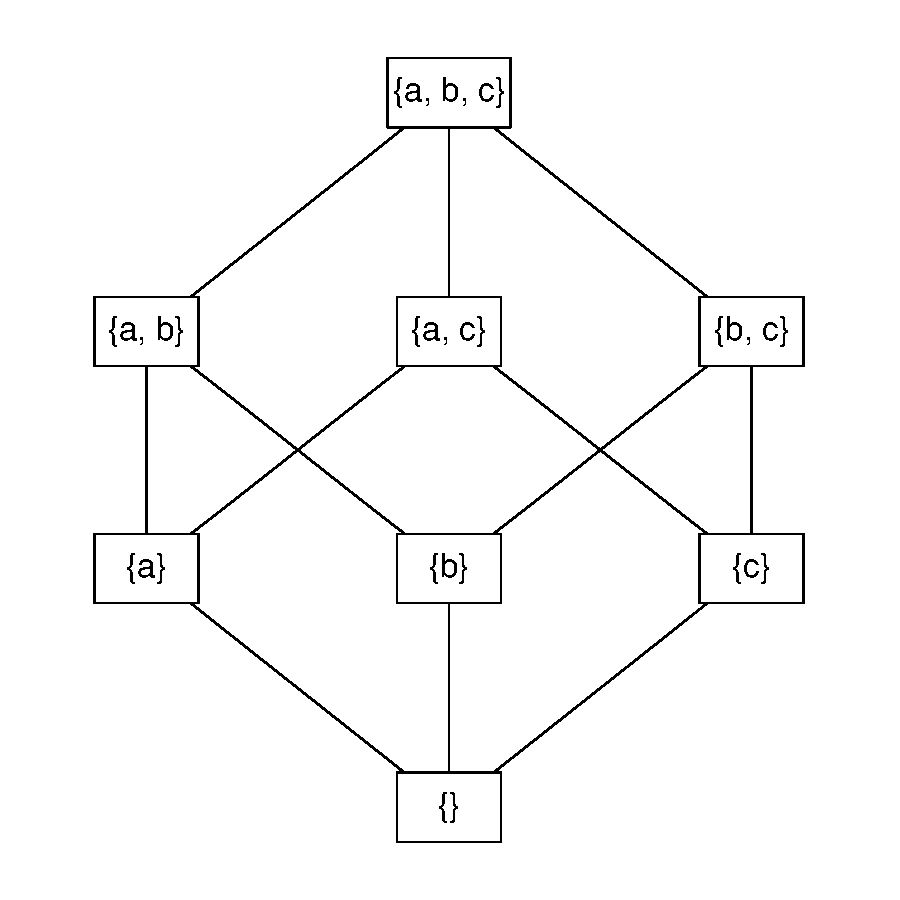
\includegraphics{relations-plotfig}
\caption{Hasse Diagram of the inclusion relation on the power set of
  $\{1,2,3\}$.}
\label{fig:plot}
\end{center}
\end{figure}

\subsection{Relational Algebra}

In addition to the basic operations defined on relations,
the package provides functionality similar to the corresponding
operations defined in relational algebra theory as introduced by
\cite{ranking:Codd:1970}.
Note, however, that domains in database relations, unlike the
concept of relations we use here, are unordered.  In fact, a database
relation (\dQuote{table}) is defined as a set of elements called
\dQuote{tuples}, where the \dQuote{tuple} components are named, but
unordered.  Thus, a \dQuote{tuple} in this Codd sense is a set of
mappings from the attribute names into the union of the attribute
domains.  The functions defined in \pkg{relations}, however, preserve
and respect the column ordering.

The \emph{projection} of a relation on a specified margin (i.e., a
vector of domain names or indices) is the relation obtained when all
tuples are restricted to this margin.  As a consequence, duplicate
tuples are removed. The corresponding function in package \pkg{relations}
is \codefunind{relation\_projection}.
\begin{Schunk}
\begin{Sinput}
> Person <- data.frame(Name = c("Harry", "Sally", "George", "Helena", 
+     "Peter"), Age = c(34, 28, 29, 54, 34), Weight = c(80, 64, 
+     70, 54, 80), stringsAsFactors = FALSE)
> Person <- as.relation(Person)
> relation_table(Person)
\end{Sinput}
\begin{Soutput}
 Name   Age Weight
 Harry  34  80    
 Peter  34  80    
 Sally  28  64    
 George 29  70    
 Helena 54  54    
\end{Soutput}
\begin{Sinput}
> relation_table(relation_projection(Person, c("Age", "Weight")))
\end{Sinput}
\begin{Soutput}
 Age Weight
 34  80    
 28  64    
 29  70    
 54  54    
\end{Soutput}
\end{Schunk}
(Note that Harry and Peter have the same age and weight.)

The \emph{selection} of a relation is the relation obtained by taking
a subset of the relation graph, defined by some logical
expression. The corresponding function in \pkg{relations} is
\codefunind{relation\_selection}.
\begin{Schunk}
\begin{Sinput}
> relation_table(R1 <- relation_selection(Person, Age < 29))
\end{Sinput}
\begin{Soutput}
 Name  Age Weight
 Sally 28  64    
\end{Soutput}
\begin{Sinput}
> relation_table(R2 <- relation_selection(Person, Age >= 34))
\end{Sinput}
\begin{Soutput}
 Name   Age Weight
 Harry  34  80    
 Peter  34  80    
 Helena 54  54    
\end{Soutput}
\begin{Sinput}
> relation_table(R3 <- relation_selection(Person, Age == Weight))
\end{Sinput}
\begin{Soutput}
 Name   Age Weight
 Helena 54  54    
\end{Soutput}
\end{Schunk}

The \emph{union} of two relations simply combines the graph elements of
both relations; the \emph{complement} of two relations $X$ and $Y$
removes the tuples of $Y$ from $X$.  One can use \codeind{-} as a
shortcut for \codefunind{relation\_complement}, and \codeind{\%U\%} or
\codeind{|} for \codefunind{relation\_union}.
The difference between \code{\%U\%}
and \code{|} is that the latter only works for identical domains.

\begin{Schunk}
\begin{Sinput}
> relation_table(R1 %U% R2)
\end{Sinput}
\begin{Soutput}
 Name   Age Weight
 Harry  34  80    
 Peter  34  80    
 Sally  28  64    
 Helena 54  54    
\end{Soutput}
\begin{Sinput}
> relation_table(R2 | R3)
\end{Sinput}
\begin{Soutput}
 Name   Age Weight
 Harry  34  80    
 Peter  34  80    
 Helena 54  54    
\end{Soutput}
\begin{Sinput}
> relation_table(Person - R2)
\end{Sinput}
\begin{Soutput}
 Name   Age Weight
 Sally  28  64    
 George 29  70    
\end{Soutput}
\end{Schunk}

The \emph{intersection} (\emph{symmetric difference}) of two relations
is the relation with all tuples they have (do not have) in common.
One can use \codeind{\&} instead of \codefunind{relation\_intersection}
in case of identical domains.

\begin{Schunk}
\begin{Sinput}
> relation_table(relation_intersection(R2, R3))
\end{Sinput}
\begin{Soutput}
 Name   Age Weight
 Helena 54  54    
\end{Soutput}
\begin{Sinput}
> relation_table(R2 & R3)
\end{Sinput}
\begin{Soutput}
 Name   Age Weight
 Helena 54  54    
\end{Soutput}
\begin{Sinput}
> relation_table(relation_symdiff(R2, R3))
\end{Sinput}
\begin{Soutput}
 Name  Age Weight
 Harry 34  80    
 Peter 34  80    
\end{Soutput}
\end{Schunk}

The \emph{Cartesian product} of two relations is obtained by basically
building the Cartesian product of all graph elements, but combining the
resulting pairs into single tuples. A shortcut for
\codefunind{relation\_cartesian} is \codeind{\%><\%}.

\begin{Schunk}
\begin{Sinput}
> Employee <- data.frame(Name = c("Harry", "Sally", "George", "Harriet", 
+     "John"), EmpId = c(3415, 2241, 3401, 2202, 3999), DeptName = c("Finance", 
+     "Sales", "Finance", "Sales", "N.N."), stringsAsFactors = FALSE)
> Employee <- as.relation(Employee)
> relation_table(Employee)
\end{Sinput}
\begin{Soutput}
 Name    EmpId DeptName
 Harry   3415  Finance 
 George  3401  Finance 
 Sally   2241  Sales   
 Harriet 2202  Sales   
 John    3999  N.N.    
\end{Soutput}
\begin{Sinput}
> Dept <- data.frame(DeptName = c("Finance", "Sales", "Production"), 
+     Manager = c("George", "Harriet", "Charles"), stringsAsFactors = FALSE)
> Dept <- as.relation(Dept)
> relation_table(Dept)
\end{Sinput}
\begin{Soutput}
 DeptName   Manager
 Finance    George 
 Sales      Harriet
 Production Charles
\end{Soutput}
\begin{Sinput}
> relation_table(Employee %><% Dept)
\end{Sinput}
\begin{Soutput}
 Name    EmpId DeptName DeptName   Manager
 Harry   3415  Finance  Finance    George 
 George  3401  Finance  Finance    George 
 Sally   2241  Sales    Finance    George 
 Harriet 2202  Sales    Finance    George 
 John    3999  N.N.     Finance    George 
 Harry   3415  Finance  Sales      Harriet
 George  3401  Finance  Sales      Harriet
 Sally   2241  Sales    Sales      Harriet
 Harriet 2202  Sales    Sales      Harriet
 John    3999  N.N.     Sales      Harriet
 Harry   3415  Finance  Production Charles
 George  3401  Finance  Production Charles
 Sally   2241  Sales    Production Charles
 Harriet 2202  Sales    Production Charles
 John    3999  N.N.     Production Charles
\end{Soutput}
\end{Schunk}

The \emph{division} of relation $X$ by relation $Y$ is the
reversed Cartesian product.  The result is a relation with the domain
unique to $X$ and containing the maximum number of tuples which,
multiplied by $Y$, are contained in $X$.  The \emph{remainder}
of this operation is the complement of $X$ and the division of
$X$ by $Y$.  Note that for both operations, the domain of
$Y$ must be contained in the domain of $X$. The shortcuts for
\codefunind{relation\_division} and \codefunind{relation\_remainder} are
\codeind{\%/\%} and \codeind{\%\%}, respectively.

\begin{Schunk}
\begin{Sinput}
> Completed <- data.frame(Student = c("Fred", "Fred", "Fred", "Eugene", 
+     "Eugene", "Sara", "Sara"), Task = c("Database1", "Database2", 
+     "Compiler1", "Database1", "Compiler1", "Database1", "Database2"), 
+     stringsAsFactors = FALSE)
> Completed <- as.relation(Completed)
> relation_table(Completed)
\end{Sinput}
\begin{Soutput}
 Student Task     
 Fred    Database1
 Eugene  Database1
 Sara    Database1
 Fred    Database2
 Sara    Database2
 Fred    Compiler1
 Eugene  Compiler1
\end{Soutput}
\begin{Sinput}
> DBProject <- data.frame(Task = c("Database1", "Database2"), stringsAsFactors = FALSE)
> DBProject <- as.relation(DBProject)
> relation_table(DBProject)
\end{Sinput}
\begin{Soutput}
 Task     
 Database1
 Database2
\end{Soutput}
\begin{Sinput}
> relation_table(Completed%/%DBProject)
\end{Sinput}
\begin{Soutput}
 Student
 Fred   
 Sara   
\end{Soutput}
\begin{Sinput}
> relation_table(Completed%%DBProject)
\end{Sinput}
\begin{Soutput}
 Student Task     
 Eugene  Database1
 Fred    Compiler1
 Eugene  Compiler1
\end{Soutput}
\end{Schunk}

The (natural) \emph{join} of two relations is their Cartesian product,
restricted to the subset where the elements of the common attributes do
match.  The left/right/full outer join of two relations $X$ and $Y$ is
the union of $X$/$Y$/($X$ and $Y$), and the inner join of $X$ and $Y$.
The implementation of \codefun{relation\_join} uses \codefun{merge}, and
so the left/right/full outer joins are obtained by setting
\code{all.x}/\code{all.y}/\code{all} to \code{TRUE} in
\codefunind{relation\_join}.
The domains to be matched are specified
using \code{by}.  Alternatively, one can use the operators
\codeind{\%|><|\%}, \codeind{\%=><\%}, \codeind{\%><=\%},
and \codeind{\%=><=\%} for the natural join, left join,
right join, and full outer join, respectively.

\begin{Schunk}
\begin{Sinput}
> relation_table(Employee %|><|% Dept)
\end{Sinput}
\begin{Soutput}
 Name    EmpId DeptName Manager
 Harry   3415  Finance  George 
 George  3401  Finance  George 
 Sally   2241  Sales    Harriet
 Harriet 2202  Sales    Harriet
\end{Soutput}
\begin{Sinput}
> relation_table(Employee %=><% Dept)
\end{Sinput}
\begin{Soutput}
 Name    EmpId DeptName Manager
 Harry   3415  Finance  George 
 George  3401  Finance  George 
 John    3999  N.N.     NA     
 Sally   2241  Sales    Harriet
 Harriet 2202  Sales    Harriet
\end{Soutput}
\begin{Sinput}
> relation_table(Employee %><=% Dept)
\end{Sinput}
\begin{Soutput}
 Name    EmpId DeptName   Manager
 Harry   3415  Finance    George 
 George  3401  Finance    George 
 NA        NA  Production Charles
 Sally   2241  Sales      Harriet
 Harriet 2202  Sales      Harriet
\end{Soutput}
\begin{Sinput}
> relation_table(Employee %=><=% Dept)
\end{Sinput}
\begin{Soutput}
 Name    EmpId DeptName   Manager
 Harry   3415  Finance    George 
 George  3401  Finance    George 
 John    3999  N.N.       NA     
 NA        NA  Production Charles
 Sally   2241  Sales      Harriet
 Harriet 2202  Sales      Harriet
\end{Soutput}
\end{Schunk}

The left (right) \emph{semijoin} of two relations $X$ and $Y$
is the join of these, projected to the attributes of $X$
($Y$). Thus, it yields all tuples of $X$
($Y$) participating in the join of $X$ and $Y$.
Shortcuts for \codefunind{relation\_semijoin} are
\codeind{\%|><\%} and \codeind{\%><|\%} for left and right
semijoin, respectively.

\begin{Schunk}
\begin{Sinput}
> relation_table(Employee %|><% Dept)
\end{Sinput}
\begin{Soutput}
 Name    EmpId DeptName
 Harry   3415  Finance 
 George  3401  Finance 
 Sally   2241  Sales   
 Harriet 2202  Sales   
\end{Soutput}
\begin{Sinput}
> relation_table(Employee %><|% Dept)
\end{Sinput}
\begin{Soutput}
 DeptName Manager
 Finance  George 
 Sales    Harriet
\end{Soutput}
\end{Schunk}

The left (right) \emph{antijoin} of two relations $X$ and $Y$
is the complement of $X$ ($Y$) and the join of both,
projected to the attributes of $X$ ($Y$). Thus, it yields all tuples
of $X$ ($Y$) \emph{not} participating in the join of $X$ and $Y$.
Shortcuts for \codefunind{relation\_antijoin} are
\codeind{\%|>\%} and \codeind{\%<|\%} for left and right antijoin, respectively.

\begin{Schunk}
\begin{Sinput}
> relation_table(Employee %|>% Dept)
\end{Sinput}
\begin{Soutput}
 Name EmpId DeptName
 John 3999  N.N.    
\end{Soutput}
\begin{Sinput}
> relation_table(Employee %<|% Dept)
\end{Sinput}
\begin{Soutput}
 DeptName   Manager
 Production Charles
\end{Soutput}
\end{Schunk}

\subsection{Relation Ensembles}

\dQuote{Relation ensembles} are collections of relations $R_i = (D,
G_i)$ with the same domain $D$ and possibly different graphs $G_i$.
Such ensembles are implemented as suitably classed lists of relation
objects (of class \class{relation\_ensemble} and inheriting from
\class{tuple}), making it possible to use \codefun{lapply} for
computations on the individual relations in the ensemble.  Relation
ensembles can be created via \codefunind{relation\_ensemble},
or by coercion via the generic function \codefunind{as.relation\_ensemble}
which has methods for at least data frames (regarding each variable as a
separate relation).  Available methods for relation ensembles include
those for subscripting, \codefun{c}, \codefun{t}, \codefun{rep}, \codefun{print}, and
\codefun{plot}.  In addition, there are summary methods defined
(\codefun{min}, \codefun{max}, and \codefun{range}).  Other operations
work element-wise like on tuples due to the inheritance.

The Cetacea data set \citep{relations:Vescia:1985} is a data frame with
15 variables relating to morphology, osteology, or behavior, with both
self-explanatory names and levels, and a common zoological
classification (variable \code{CLASS}) for 36 types of cetacea.  We
consider each variable an equivalence relation on the objects, excluding
2 variables with missing values, giving a relation ensemble of length 14
(number of complete variables in the data set).
\begin{Schunk}
\begin{Sinput}
> data("Cetacea")
> ind <- sapply(Cetacea, function(s) all(!is.na(s)))
> relations <- as.relation_ensemble(Cetacea[, ind])
> print(relations)
\end{Sinput}
\begin{Soutput}
An ensemble of 14 relations of size 36 x 36.
\end{Soutput}
\end{Schunk}
Available methods for relation ensembles allow to determine duplicated
(relation) entries, to replicate and combine, and extract unique
elements:
\begin{Schunk}
\begin{Sinput}
> any(duplicated(relations))
\end{Sinput}
\begin{Soutput}
[1] FALSE
\end{Soutput}
\begin{Sinput}
> thrice <- c(rep(relations, 2), relations)
> all.equal(unique(thrice), relations)
\end{Sinput}
\begin{Soutput}
[1] "names for current but not for target"
\end{Soutput}
\end{Schunk}
Note that \codefun{unique} does not preserve attributes, and hence
names.  In case one wants otherwise, one can subscript by a logical
vector indicating the non-duplicated entries:
\begin{Schunk}
\begin{Sinput}
> all.equal(thrice[!duplicated(thrice)], relations)
\end{Sinput}
\begin{Soutput}
[1] TRUE
\end{Soutput}
\end{Schunk}

Relation (cross-)dissimilarities can be computed for relations and
ensembles thereof:
\begin{Schunk}
\begin{Sinput}
> relation_dissimilarity(relations[1:2], relations["CLASS"])
\end{Sinput}
\begin{Soutput}
                 CLASS
NECK               584
FORM_OF_THE_HEAD   330
\end{Soutput}
\end{Schunk}
To determine which single variable is \dQuote{closest} to the zoological
classification:
\begin{Schunk}
\begin{Sinput}
> d <- relation_dissimilarity(relations)
> sort(as.matrix(d)[, "CLASS"])[-1]
\end{Sinput}
\begin{Soutput}
                         BLOW_HOLE                         DORSAL_FIN 
                               190                                240 
                      SET_OF_TEETH                           FLIPPERS 
                               288                                298 
                  FORM_OF_THE_HEAD                            FEEDING 
                               330                                382 
                           HABITAT                               BEAK 
                               398                                456 
                             COLOR LONGITUDINAL_FURROWS_ON_THE_THROAT 
                               494                                506 
                CERVICAL_VERTEBRAE                   SIZE_OF_THE_HEAD 
                               508                                542 
                              NECK 
                               584 
\end{Soutput}
\end{Schunk}

There is also an Ops group method for relation ensembles which works
elementwise (in essence, as for tuples):
\begin{Schunk}
\begin{Sinput}
> complement <- !relations
> complement
\end{Sinput}
\begin{Soutput}
An ensemble of 14 relations of size 36 x 36.
\end{Soutput}
\end{Schunk}

\section{Consensus Relations}
\label{sec:consensus}

Consensus relations \dQuote{synthesize} the information in the
elements of a relation ensemble into a single relation, often by
minimizing a criterion function measuring how dissimilar consensus
candidates are from the (elements of) the ensemble (the so-called
\dQuote{optimization approach}), typically of the form
$L(R) = \sum w_b d(R_b, R)$, where $d$ is a suitable
dissimilarity measure  and
$w_b$ is the case weight given to element $R_b$ of the
ensemble \cite[such consensus relations are called \dQuote{central
  relations} in][]{ranking:Regnier:1965}.

Consensus relations can be computed by \codefunind{relation\_consensus},
which has the following built-in methods.  Apart from Condorcet's, these
are applicable to ensembles of endorelations only.
\begin{description}
 \item[\code{"Borda"}] the consensus method proposed by
  \cite{ranking:Borda:1781}.  For each relation $R_b$ and object $x$,
  one determines the Borda/Kendall scores, i.e., the number of objects
  $y$ such that $y R_b x$ (\dQuote{wins} in case of orderings).
  These are then aggregated across relations
  by weighted averaging.  Finally, objects are ordered according to
  their aggregated scores.
 \item[\code{"Copeland"}] the consensus method proposed by
  \cite{ranking:Copeland:1951} is similar to the Borda method, except
  that the Copeland scores are the number of objects
  $y$ such that $y R_b x$, minus the number of objects
  $y$ such that $x R_b y$ (\dQuote{defeats} in case of orderings).
 \item[\code{"Condorcet"}] the consensus method proposed by
  \cite{ranking:Condorcet:1785}, in fact minimizing the criterion
  function $L$ with $d$ as symmetric difference distance over all
  possible relations.  In the case of endorelations, consensus is
  obtained by weighting voting, such that $x R y$ if the weighted number
  of times that $x R_b y$ is no less than the weighted number of times
  that this is not the case.  Even when aggregating linear orders, this
  can lead to intransitive consensus solutions (\dQuote{effet
    Condorcet}).
 \item[\code{"SD/\var{F}"}]an exact solver for determining the
    consensus relation by minimizing the criterion function $L$ with $d$
    as symmetric difference distance (\dQuote{SD}) over a suitable
    class (\dQuote(Family)) of endorelations as
    indicated by \var{F}, with values:
    \begin{description}
     \item[\code{E}] equivalence relations: reflexive, symmetric, and
        transitive.
     \item[\code{L}] linear orders: complete (hence reflexive),
        antisymmetric, and transitive.
     \item[\code{O}] partial orders: reflexive, antisymmetric and
        transitive.
     \item[\code{P}] complete preorders (preference relations,
        \dQuote{orderings}): complete (hence reflexive) and transitive.
     \item[\code{T}] tournaments: complete (hence reflexive) and
        antisymmetric.
     \item[\code{C}] complete relations.
     \item[\code{A}] antisymmetric relations.
     \item[\code{S}] symmetric relations.
    \end{description}
    These consensus relations are determined by reformulating the
    consensus problem as an integer program (for the relation
    incidences), which is solved via package \pkg{lpSolve}.  See
    \cite{ranking:Hornik+Meyer:2007} for details.
\end{description}

In the following, we first show an example of computing a consensus
equivalence (i.e., a consensus partition) of 30 felines repeating the
classical analysis of \cite{ranking:Marcotorchino+Michaud:1982}.  The
data comprises 10 morphological and 4 behavioral variables, taken here
as different classifications of the same 30 animals:

\begin{Schunk}
\begin{Sinput}
> data("Felines")
> relations <- as.relation_ensemble(Felines)
\end{Sinput}
\end{Schunk}
Now fit an equivalence relation to this, and look at the classes:
\begin{Schunk}
\begin{Sinput}
> E <- relation_consensus(relations, "SD/E")
> ids <- relation_class_ids(E)
> split(rownames(Felines), ids)
\end{Sinput}
\begin{Soutput}
$`1`
[1] "LION"  "TIGRE"

$`2`
[1] "JAGUAR"  "LEOPARD" "ONCE"    "PUMA"    "NEBUL"   "LYNX"   

$`3`
[1] "GUEPARD"

$`4`
 [1] "SERVAL"   "OCELOT"   "CARACAL"  "VIVERRIN" "YAGUARUN" "CHAUS"   
 [7] "DORE"     "MERGUAY"  "MARGERIT" "CAFER"    "CHINE"    "BENGALE" 
[13] "ROUILLEU" "MALAIS"   "BORNEO"   "NIGRIPES" "MANUL"    "MARBRE"  
[19] "TIGRIN"   "TEMMINCK" "ANDES"   
\end{Soutput}
\end{Schunk}
Next, we demonstrate the computation of consensus preferences, using an
example from
\citet[pp.~48ff]{ranking:Cook+Kress:1992}.  The input data is a
\dQuote{preference} matrix of paired comparisons, which we first
transform into a tournament.
\begin{Schunk}
\begin{Sinput}
> pm <- matrix(c(0, 1, 0, 1, 1, 0, 0, 0, 1, 1, 1, 1, 0, 0, 0, 0, 
+     0, 1, 0, 0, 0, 0, 1, 1, 0), nr = 5, byrow = TRUE, dimnames = list(letters[1:5], 
+     letters[1:5]))
> R <- as.relation(1 - pm)
> relation_incidence(R)
\end{Sinput}
\begin{Soutput}
Incidences:
  a b c d e
a 1 0 1 0 0
b 1 1 1 0 0
c 0 0 1 1 1
d 1 1 0 1 1
e 1 1 0 0 1
\end{Soutput}
\begin{Sinput}
> relation_is_tournament(R)
\end{Sinput}
\begin{Soutput}
[1] TRUE
\end{Soutput}
\end{Schunk}
Next, we seek a linear consensus order:
\begin{Schunk}
\begin{Sinput}
> L <- relation_consensus(R, "SD/L")
> relation_incidence(L)
\end{Sinput}
\begin{Soutput}
Incidences:
  a b c d e
a 1 0 1 0 0
b 1 1 1 0 0
c 0 0 1 0 0
d 1 1 1 1 1
e 1 1 1 0 1
\end{Soutput}
\end{Schunk}
or perhaps more conveniently, the class ids sorted according to
increasing preference:
\begin{Schunk}
\begin{Sinput}
> relation_class_ids(L)
\end{Sinput}
\begin{Soutput}
a b c d e 
4 3 5 1 2 
\end{Soutput}
\end{Schunk}
Note, however, that this linear order is not unique; we can compute
\emph{all} consensus linear orders, and also produce a comparing plot
(see Figure~\ref{fig:plot2}):
\begin{Schunk}
\begin{Sinput}
> L <- relation_consensus(R, "SD/L", control = list(all = TRUE))
> print(L)
\end{Sinput}
\begin{Soutput}
An ensemble of 2 relations of size 5 x 5.
\end{Soutput}
\begin{Sinput}
> if (require("Rgraphviz")) plot(L)
\end{Sinput}
\end{Schunk}
Finally, we compute the closest preference relation with at most 3
indifference classes:
\begin{Schunk}
\begin{Sinput}
> P3 <- relation_consensus(R, "SD/P", control = list(k = 3))
> relation_incidence(P3)
\end{Sinput}
\begin{Soutput}
Incidences:
  a b c d e
a 1 0 0 0 0
b 1 1 0 0 1
c 1 1 1 1 1
d 1 1 1 1 1
e 1 1 0 0 1
\end{Soutput}
\begin{Sinput}
> relation_class_ids(P3)
\end{Sinput}
\begin{Soutput}
a b c d e 
3 2 1 1 2 
\end{Soutput}
\end{Schunk}
(Note again that this preference is not unique; there are 6 consensus
preferences with $k = 3$ classes, which can be computed as above by
adding \code{all = TRUE} to the \code{control} list.)

\begin{figure}[h]
\begin{center}
\includegraphics{relations-consensusfig}
\caption{Hasse Diagram of all consensus relations (linear orders) for an
  example provided by Cook and Kress.}
\label{fig:plot2}
\end{center}
\end{figure}

% \section{Outlook}
% \label{sec:outlook}

% In addition to the dQuote{crisp} relations descrbied,
% there is also the notion of fuzzy relations, for which each tuple is
% contained in the graph with a certain membership value.  (I.e., the
% graph is a fuzzy subset of the Cartesian product of the elements of
% the domain.) Basic support for fuzzy relations will be added
% eventually.

% \subsubsection*{Acknowledgments}

% We are grateful to Walter B\"ohm for providing efficient C code for
% solving assignment problems.

{\small
  \bibliographystyle{abbrvnat}
  \bibliography{relations}
}

\printindex{}

\end{document}
